
 \documentclass{article}
\usepackage{amsmath}
% if you need to pass options to natbib, use, e.g.:
% \PassOptionsToPackage{numbers, compress}{natbib}
% before loading nips_2017
%
% to avoid loading the natbib package, add option nonatbib:
% \usepackage[nonatbib]{nips_2017}

%\usepackage{nips_2017}

% to compile a camera-ready version, add the [final] option, e.g.:
\usepackage[final]{nips_2017}

\usepackage[utf8]{inputenc} % allow utf-8 input
\usepackage[T1]{fontenc}    % use 8-bit T1 fonts
\usepackage{hyperref}       % hyperlinks
\usepackage{url}            % simple URL typesetting
\usepackage{booktabs}       % professional-quality tables
\usepackage{amsfonts}       % blackboard math symbols
\usepackage{nicefrac}       % compact symbols for 1/2, etc.
\usepackage{microtype}      % microtypography
\usepackage{subfig}
\usepackage{cleveref}
\usepackage{graphicx}
\usepackage{siunitx}

\graphicspath{ {hw4/imgs/} }

\title{Computer Vision 1: Final Project - part 2}


\author{
	Gabriele Bani \\
	11640758 \\
  \texttt{gabriele.bani@student.uva.nl} \\
  %% examples of more authors
  \And
  	Andrii Skliar \\
  11636785 \\
  \texttt{andrii.skliar@student.uva.nl} \\
}

\begin{document}
\maketitle

\section{Introduction}

We also analyze CNN architectures and understand their behavior under different hyperparameter settings. We explore how a pretrained network can be used on another dataset in order to achieve good results, without occurring in overfitting or underfitting behaviors, thanks to fine tuning procedures. We evaluate both qualitatively and quantitatively the features from the pre trained model and the fine tuned model, and show how fine tuning constantly produces superior results. Finally, we apply different additional variations to the training procedures and analyze their effects.  

\section{Understanding the Network Architecture}



The network can be logically divided in 5 blocks, and clearly shows a pattern. Every block contains a convolutional layer, and apart the last block, they also all have a pooling layer. It would make no sense in fact to apply a further pooling at this point since the size of the data is already 1 in the first two dimensions. 
Also, apart from the first and last block, we have a ReLU non-linearity after the convolution in the same block. In the last layer, it is reasonable to not include the non linearity since we want to output probabilities, and thus apply a softmax. So, the most frequent pattern seen in this network is (conv, relu*, pool), repeated many times in the network, where we put the star on relu because there is one exception in which it is not present.


Pooling layers and non-linearity layers have no parameters. Since parameters are shared, convolutional layers have a number of parameters equal to $d \times d \times F_i \times F_o$, where $d$ is the size of the filter, $F_i$ is the number of input filters (from the previous layer), and $F_o$ is the number of output filters of the conv layer. So, by looking at our architecture, the layer with most parameters is layer 10 (the second-to last conv layer), with $4 \times 4 \times 64 \times 64 = 65536$ weights. To compute the memory consumption, this value has to be multiplied by 4, since every weight is represented by a 32 bit floating point number, and we obtain the same value reported in \cref{fig:memtable}, $256$ KB (in the row "param mem"). 

The memory needed for a convolutional layer is given by $I \times I \times F_o$, where $I$ is the dimension of the data and $f_o$ is the number of output filters of the layer. We can calculate the sizes of the filters and see that, as seen in \cref{fig:memtable}, the first conv layer occupies the most memory, $128$ KB per image.


\begin{figure}[h]
    \centering
    \caption{Pretrained network information}
    \subfloat{{
    	\includegraphics[width=1\textwidth]{hw5/imgs/memtable.png}
    }}
\label{fig:memtable}
\end{figure}

\section{Preparing the Input Data}

We implemented the function getCaltechIMDB as described by the requirements. Regarding the $4D$ matrix imdb.images.data, we scale every input image to $32$ by $32$ (with 3 color channels), since otherwise the images would have different width and height. The rest of the data structure is created as required.

\section{Updating the Network Architecture}

Since Block-5 of the network outputs 64 filters, NEW\_INPUT\_SIZE has to be 64.
We set NEW\_OUTPUT\_SIZE to 4 since we want to predict one probability for each of the four classes that we are considering. %The information contained in the 64 (1 by 1) filters is so combined linearly by this convolutional layer 

\section{Setting up Hyperparameters}

We run the experiments using the default hyperparameters specified in the source files and the suggested batch sizes (50, 100) and epochs number (40, 80, 120). We report in \cref{tab:restab} the results at the end of the training, and in \cref{fig:results} the respective training curves. These results are all very impressive, with the lowest validation errors being of just one percent. Batch size seems to have an impact on the training, making the losses decrease more slowly. Even though this might affects the evaluation metric on other situations, in our case the training and validation errors are so low that we cannot make reliable conclusions about them. The number of epochs affects mainly the value of the loss function, since the training accuracies are so high that no meaningful deductions can be made from them.

Finally, we kept the model with highest accuracy on the validation set. Since multiple models have the same validation accuracy, we kept the first one found, which in our case was with batch size $50$ for $40$ epochs. Even though it is clearly not the best in term of loss, we kept it as best model in order to keep consistency in the code. Results in the bonus part will be based on this model. 

\begin{figure}[h]
    \centering
    \caption{Training curves with different batch sizes and epochs}
    \subfloat[Batch size 50 - 40 epochs]{{
    	\includegraphics[width=0.3\textwidth]{hw5/imgs/50-402.jpg}
    }}
    \subfloat[Batch size 50 - 80 epochs]{{
    	\includegraphics[width=0.3\textwidth]{hw5/imgs/50-802.jpg}
    }}
    \subfloat[Batch size 50 - 120 epochs]{{
    	\includegraphics[width=0.3\textwidth]{hw5/imgs/50-1202.jpg}
    }}\\
    \subfloat[Batch size 100 - 40 epochs]{{
    	\includegraphics[width=0.3\textwidth]{hw5/imgs/100-402.jpg}
    }}
    \subfloat[Batch size 100 - 80 epochs]{{
    	\includegraphics[width=0.3\textwidth]{hw5/imgs/100-802.jpg}
    }}
    \subfloat[Batch size 100 - 120 epochs]{{
    	\includegraphics[width=0.3\textwidth]{hw5/imgs/100-1202.jpg}
    }}\\
\label{fig:results}
\end{figure}


\begin{table}
	\centering
	\captionsetup{justification=centering}
	\renewcommand{\arraystretch}{1.5}
	\setlength{\abovecaptionskip}{15pt plus 3pt minus 2pt} % Chosen fairly arbitrarily
	\begin{tabular}{|c|c|c|c|c|c|c|c|c|c|c|c|c|c|c|c|c|c|}
		\hline
		& \multicolumn{3}{c|}{\textbf{Train loss}} & \multicolumn{3}{c|}{\textbf{Train err}} & \multicolumn{3}{c|}{\textbf{Val loss}} & \multicolumn{3}{c|}{\textbf{Val err}} \\
		% \hline
		% \textbf{Inactive Modes} & \textbf{Description}\\
		\cline{2-13}
		& \textbf{40 ep} & \textbf{80 ep} & \textbf{120 ep} & \textbf{40 ep} & \textbf{80 ep} & \textbf{120 ep} & \textbf{40 ep} & \textbf{80 ep} & \textbf{120 ep} & \textbf{40 ep} & \textbf{80 ep} & \textbf{120 ep}  \\
		%\hhline{~--}
		\hline
	Batch size 50          & 0.35 & 0.056 & 0.037 & 0.054 & 0 & 0 & 1.03 & 0.93 & 1.10 & 0.50 & 0.50 & 1.00 \\ \hline
	Batch size 100          & 1.49 & 0.26 & 0.15 & 0.27 & 0 & 0 & 2.83 & 1.94 & 1.36 & 1.00 & 0.50 & 0.50 \\ \hline
	
	\end{tabular}
    \caption{Results under different settings - all the values are divided by 100 for better visualization}
	\label{tab:restab}
\end{table}

\section{Feature space visualization}

\begin{figure}[h]
    \centering
    \caption{Tsne low dimensional visualization}
    \subfloat[Pretrained features visualization]{{
    	\includegraphics[width=0.5\textwidth]{hw5/imgs/tsne_pre.jpg}
    }}
    \subfloat[Finetuned features visualization]{{
    	\includegraphics[width=0.5\textwidth]{hw5/imgs/tsne_fine.jpg}
    }}
\label{fig:tsne}
\end{figure}

We extract features from the two networks before the last layer, skipping the relu activation as done in the script train\_svm.m. In general, features are considered as the neuron activations, which means, that they include the nonlinearity. To keep consistency with the given code, we however ignore the relu. Anyways, in this simple setting the results are qualitatively very similar in either case.

From \cref{fig:tsne} we can see a clear difference in the visualization of the feature spaces in the two cases. In the pretrained model, the data points are spread in the feature space without clearly forming separable clusters. Without label coloring, it would be difficult even for a human to separate the data clearly in clusters. We can see however that most of the faces are close to each other, while all the other classes are much more spread out and overlapping. On the other side, we clearly see a completely opposite situation in the feature space visualization of the finetuned features. The data is clearly divided in 4 major clusters, even though minor clusters are still present. A human in this case could clearly identify the four major clusters with no problem. The problem of overlapping is almost completely removed (only a few outliers are found in other classes clusters). This means that given a datapoint, we can be almost sure that the neighboring datapoints are of the same class, which is a very good indicator that the network understands the main characteristics of the data.

\subsection{Evaluating Accuracy}

We measure the accuracies using the three configurations, and obtain 99.50 $\%$ for the finetuned model, 89.50 $\%$ for the SVM using the pretrained model features and 99.50 $\%$ using SVM with the finetuned model features. We can see from these results that the pretrained model was not able to model well enough the new data, while the finetuned model could. In fact, it could not only achieve high accuracy by itself, but also allowed the SVM to achieve almost the same accuracy when using its features. This could mean that the pretrained network did not generalize well enough, or that the datasets used is significantly different from the one used to pretrain it. We suggest the second option, since pretrained accuracy is still pretty high, almost $90\%$.

Comparing with the results obtained in the first part of the homework, where we used hand crafted features with the bag of words approach, we obtain much better results, with much less effort. In the previous part, many parameters had to be set empirically, and some of those had much more relevance than others (vocabulary size, color space, SIFT type). These regard the kind of features that will be used, and are typically dataset dependent. So, whenever we want to analyze a new dataset, we have to search again for good configuration of parameters, knowing that even one wrong choice could lead to poor results (see RBF kernel in our case). Although training a neural network from scratch might be also hard, nowdays there are plenty of pretrained models available, especially in computer vision. When fine tuning, the advantages of using neural networks become overwhelming. The number of parameters needed for fine tuning is much lower, since the architecture of the network is already decided. Also, transfer learning can be used even for different tasks easily, while other approaches typically do not allow this. Although the main advantage of hand crafted features and the bag of words approach is that they can work well with small amount of data, we have shown here that by fine tuning a pretrained model, we can achieve even better results even with small datasets.
To conclude, neural networks provide a consistent way to extract knowledge from data and allow to achieve the best results in many different situations, and using hand crafted features typically does not pay off in both easy of use and results obtained.

\section{Improvements (Bonus part)}
\subsection{Data augmentation}

\begin{table}
	\centering
	\captionsetup{justification=centering}
	\renewcommand{\arraystretch}{1.5}
	\setlength{\abovecaptionskip}{15pt plus 3pt minus 2pt} % Chosen fairly arbitrarily
	\begin{tabular}{|c|c|c|c|c|c|c|c|c|c|c|c|c|c|c|c|c|c|}
		\hline
		& \textbf{CNN classification} & \textbf{SVM on finetuned features}  \\
		%\hhline{~--}
		\hline
	Original          & 99.50 & 99.50  \\ \hline
	Only noise          & 98.50 & 97.50  \\ \hline
	Only rotation          & 99.00 & 98.50  \\ \hline
	Noise + rotation          & 95.00 & 97.00  \\ \hline
	Freezing layers          & 97.00 & 95.00  \\ \hline

	\end{tabular}
    \caption{Accuracies under different situations}
	\label{tab:res_augment}
\end{table}

For this part, we execute two different experiments. First, we introduce gaussian and salt and pepper noise. We do not create a new dataset, but randomly (and independently) apply them with probability $0.5$ for every batch. The goal of this kind of data augmentation is to make the network more robust to noise, since during trained it tries to learn to classify even when the images are noisy. We set the sigma parameter for gaussian to $0.01$, and it can be interpreted as the width of the filter. We set salt and pepper parameter to $0.05$, which means that on average, $5\%$ of the pixels will be modified.

We also apply rotation as data augmentation. Since the imrotate function can change dramatically the image with black pixels, we restrict the rotation angle between $-20$ and $20$ degrees. As before, the rotation happens with probability $0.5$, while the rotation angle is chosen uniformly between $-20$ and $20$.

finally, we apply noise and rotation. Since this made the training very unstable, we lowered the probability of rotation to $0.2$. All the results can be seen in \cref{tab:res_augment}, while the training curves can be seen in \cref{fig:augment}

The main interesting point to analyze is the behavior of the training curves, which is much different from what seen in the previous experiments. We see in fact that all our data augmentation make the learning process more difficult, with the training and even more validation curves showing wiggling behaviors. We realize that the most extreme wiggles happen when rotation is present when the highest angles are chosen. Overall, data augmentation lead to slightly worse test accuracies, in particolar when combined together. However, the models produced are now capable of better dealing with noise and rotation, which could be a desirable features in many situations.

\subsection{Freezing the layers}

\begin{figure}[h]
    \centering
    \caption{Training curves with different data augmentation}

    \subfloat[Noise]{{
    	\includegraphics[width=0.3\textwidth]{hw5/imgs/noise.jpg}
    }}
    \subfloat[Rotation]{{
    	\includegraphics[width=0.3\textwidth]{hw5/imgs/rotate.jpg}
    }}
    \subfloat[Noise and rotation]{{
    	\includegraphics[width=0.3\textwidth]{hw5/imgs/noise_rotate.jpg}
    }}
\label{fig:augment}
\end{figure}

Freezing all the layers of the network in our case leads to poor validation results (0.35 validation error) since the network cannot produce features that explain well the new dataset, so we choose to use a less invasive freezing for this task. We freeze the first two conv layers by setting their learning rate to zero, and set the next two conv layers with one tenth of the default learning rate. For the last layer we stick to to the default learning rate. The reason for this is that we assume the early layers to capture general low level features, while allow the middle layers to slowly adjust to the characteristics of the new dataset. The last conv layers still keeps the default learning rate because it is where we want most of the learning to happen, at high level.

We run one experiment, with batch size $50$ for $40$ epochs, and the results can be seen in \cref{tab:res_augment}. This performance drop respect to the fully finetuned model suggests us that the features caputred in the first layers are not general enough and cannot represent at best general features of images.

\begin{figure}[h]
    \centering
    \caption{Training curves when freezing layers}

    \subfloat{{
    	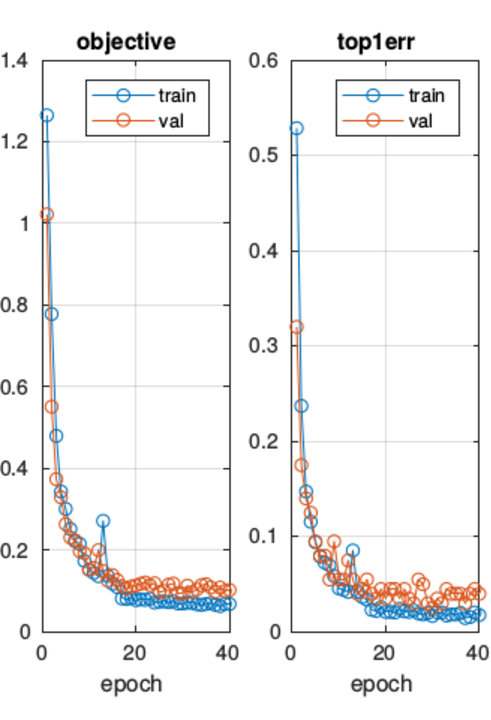
\includegraphics[width=0.3\textwidth]{hw5/imgs/freeze-50-40.jpg}
    }}
\label{fig:augment}
\end{figure}

\section{Conclusion}

We have explored how CNNs behave when used for transfer learning, and argued about their advantages over traditional feature extractors, providing empirical results. We have implemented and experimented different variations of the training proecdure, and shown how fine tuning can be harder when using data augmentation, and how freezing layers might lead to lower performance if the features extracted by the pretrained network are not general enough.

\end{document}
 